\section{Durchführung}
\label{sec:Durchführung}
\begin{figure}[H]
    \centering
    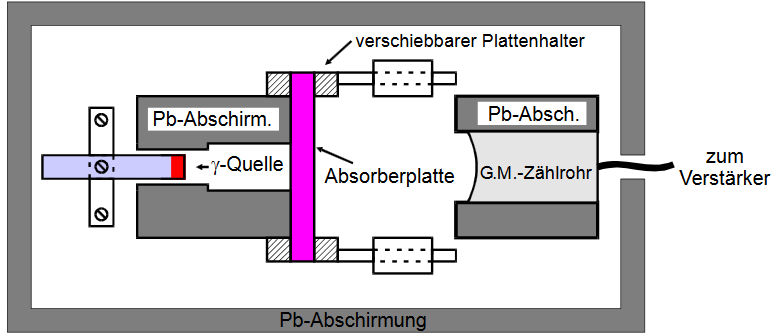
\includegraphics[width=\textwidth]{content/Aufbau.png}
    \caption{Aufbau des Versuchs. \cite{v704}}
    \label{fig:mess}
\end{figure}
\noindent
Der Versuch wird nach Abbildung \ref{fig:mess} aufgebaut.
Dabei ist zu beachten, dass für  den jeweiligen Strahler verschiedene Abschirmungen verwendet werden.
Eine dünne Aluminiumschicht für den $\beta$-Strahler und Blei für den $\gamma$-Strahler.
Die Messung wird mit einem Geiger-Müller-Zählrohr durchgeführt.
Bei diesem muss der Nulleffekt beachtet werden, dafür wird eine Messung von 900 Sekunden ohne Strahler durchgeführt.
Der Strahler wird danach ohne Absorptionsplatten, ähnlich der Messung des Nulleffekts, untersucht.
Die Dicke der Absorptionsplatten wird für die jeweiligen Materialien langsam gesteigert, dabei wird die Messzeit an die jeweiligen Wandstärken der Absorptionsplatten angepasst.
